

%\newcommand*{\ACM}{}%

\ifdefined\ACM

%\documentclass[sigplan,screen]{acmart}
  \documentclass[manuscript,screen,review]{acmart}

\else
  \documentclass{article}
  \usepackage[utf8]{inputenc}
\usepackage[a4paper, total={6in, 9in}]{geometry}
\usepackage{braket}
\usepackage{xcolor}
\usepackage{amsmath}
\usepackage{amsfonts}
\usepackage{amsthm}
\usepackage{amssymb}
%\usepackage[ocgcolorlinks]{hyperref}
\usepackage{hyperref}
%\usepackage{hyperref,xcolor}
%\usepackage[ocgcolorlinks]{ocgx2}
\usepackage{cleveref}
\usepackage{graphicx}
\usepackage{svg}
\usepackage{float}
\usepackage{tikz}
\usetikzlibrary{patterns, shapes.arrows}
\usepackage{adjustbox}
%\usepackage{tikz-network}
\usepackage{tkz-graph}
\usepackage{tkz-berge}
\usepackage[linesnumbered]{algorithm2e}
\usepackage{multicol}
\usepackage[backend=biber,style=alphabetic,sorting=ynt]{biblatex}
%\usepackage{xcolor}
%\usepackage{tkz-berge}
%\usepackage{tkz-graph}
\usepackage{pgfplots}
\usepackage{sagetex}
\usepackage{setspace}
\usepackage{etoc}
%\usepackage{wrapfig}
\usepackage{pgfgantt}
\DeclareUnicodeCharacter{2212}{−}
\usepgfplotslibrary{groupplots,dateplot}
\pgfplotsset{compat=newest}

\newtheorem{theorem}{Theorem}
\newtheorem{definition}{Definition}
\newtheorem{example}{Example}
\newtheorem{claim}{Claim}
\newtheorem{fact}{Fact}
\newtheorem{remark}{Remark}
\newtheorem*{theorem*}{Theorem}
\newtheorem{lemma}{Lemma}
\crefname{lemma}{Lemma}{Lemmas}
\hypersetup{colorlinks=true}
% , allcolors=blue,allbordercolors=blue,pdfborderstyle={0 0 1}}
%\hypersetup{pdfborder={2 2 2}}
% pdfpagemode=FullScreen,
% backref 

\newtheorem{problem}{Problem}
\crefname{problem}{Problem}{Problems}

\DeclareMathOperator{\Ima}{Im}


  \addbibresource{./sample.bib} 

\fi

\begin{document}
\newcommand{\commentt}[1]{\textcolor{blue}{ \textbf{[COMMENT]} #1}}
\newcommand{\ctt}[1]{\commentt{#1}}
\newcommand{\prb}[1]{ \mathbf{Pr} \left[ #1 \right]}
\newcommand{\prbm}[2]{ \mathbf{Pr}_{ #2 }\left[ #1 \right]}
\newcommand{\prbc}[3]{ \mathbf{Pr}_{ #2 }\left[ #1 \right | #3]}
\newcommand{\prbcprb}[3]{ \prbc{#2}{#1}{#3} \cdot \prb{#3} } 
\newcommand{\expp}[1]{ \mathbf{E} \left[ {#1} \right]}
\newcommand{\onotation}[1]{\(\mathcal{O} \left( {#1}  \right) \)}
\newcommand{\ona}[1]{\onotation{#1}}
\newcommand{\PSI}{{\ket{\psi}}}
\newcommand{\xij} { X_{ij} } 
\DeclareMathOperator{\Ima}{Im}
%\newcommand{\LESn}{\ket{\psi_n}}
%\newcommand{\LESa}{\ket{\phi_n}}
%\newcommand{\LESs}{\frac{1}{\sqrt{n}}\sum_{i}{\ket{\left(0^{i}10^{n-i}\right)^{n}}}}
%\newcommand{\Hn}{\mathcal{H}_{n}}
%\newcommand{\Ep}{\frac{1}{\sqrt{2^n}}\sum^{2^n}_{x}{ \ket{xx}}}
%\newcommand{\HON}{\ket{\psi_{\text{honest}}}}
%\newcommand{\Lemma}{\paragraph{Lemma.}}
\newcommand{\Cpa}{[n, \rho n, \delta n]}
%\setlength{\columnsep}{0.6cm}
\newcommand{\Jvv}{ \bar{J_{v}} } 
\newcommand{\Cvv}{ \tilde{C_{v}} } 

\newcommand{\Gz}{ G_{z}^{\delta} } 
\newcommand{ \Tann } {  \mathcal{T}\left( G, C_0 \right) }
\newcommand{\ireducable}{ireducable \hyperref[ire]{[\ref{ire}]} }
\newcommand{\cutUU}{E(U_{-1} \bigcup U_{+1} ,U)} 
\newcommand{\wcutUU}{w\left( E(U_{-1} \bigcup U_{+1} ,U)  \right)}
\newcommand{\testgo}{  \mathcal{T}\left(J, q , C_{0}\right) } 

\newcommand{\duC}{\left( C_{A}^{\perp}\otimes C_{B}^{\perp} \right)^{\perp}}
\newcommand{\duduC}{\left( C_{A}\otimes C_{B}\right)^{\perp}}
  




\title{Magic States Distillation  Using $\Delta$-Toric (good qLDPC?). } 
\author{David Ponarovsky}
\maketitle

%\begin{abstract}
%  We studies the complexity of synthesis quantum states using PRS, our reasch continues the work by \cite{searchtodecision}, \cite{rosenthal2023efficient}, \cite{rosenthal2021interactive}, \cite{metger2023stateqip}, \cite{delavenne2023quantum}.
%\end{abstract}
%

Let $\ket{f}$ be a codeword in $C_{X}$, and let $X_{g}$ be the indicator that equals $1$ if $f$ has support on $X_{g}$, and $0$ otherwise. Observes that applying $T^{\otimes}$ on $\ket{f}$ yilds the state: 
\begin{equation*}
  \begin{split}
    T^{\otimes n}\ket{f} & =  T^{\otimes n}\ket{\sum_{g} X_{g}g } = \exp \Big( i\pi/4 \sum_{g} X_{g}|g|  -  2 \cdot i \pi/4 \sum_{g,h} X_{g}X_{h}|g\cdot h| \\
    & +  4 \cdot i\pi/4 \sum_{g,h} X_{g}X_{h}X_{l}|g\cdot h \cdot l| -   8  \cdot i\pi/4 \cdot \text{ integers } \Big) \ket{f} \\
    & = \exp \Big( i\pi/4 \sum_{g} X_{g}|g|  -  2 \cdot \pi/4 \sum_{g,h} X_{g}X_{h}|g\cdot h| +  4 \cdot i\pi/4 \sum_{g,h} X_{g}X_{h}X_{l}|g\cdot h \cdot l| \Big) \ket{f}
  \end{split}
\end{equation*}

\section{Many to One.}
Assume that $f$ is supported on exactly one generator. Then we have that $T^{\otimes n}\ket{f}  = e^{i\pi|g|/4}\ket{f}$ Therefore, if $|g| = 4k+1$ then we are done.


\section{Using Quntum Error Correction Codes.}

Now assume that the code $C_{X}$ is the quantum Tanner code, denote by $G,A,B$ the group and the two generator sets that are used for constructing the square complex. 

\begin{claim} 
Consider $g,h$ that are supported on the same $v\in V$. We will call such a pair a source-sharing pair. Suppose that for any we have that $|g \cdot h|$ is even. Then there is a Clifford gate that computes $\ket{f} \mapsto \exp \Big(  -  i\pi \sum_{g,h \text{ source-sharing }} X_{g}X_{h}|g\cdot h|  \Big) \ket{f} $.
\end{claim}

%\begin{claim}
%  \label{claim:phase}
%  The gate $\ket{f} \mapsto \exp \Big(   i\pi \sum_{g,h} X_{g}X_{h}X_{l}|g\cdot h \cdot l| \Big) \ket{f} $ is in the Clifford group.  
%\end{claim}
%
%\begin{proof}
%  Just decode $f$ and apply \textbf{CCZ} between any triple of qubits corresponding to the generators $g,h,l$ such that $g \cdot h \cdot l=_{2} 1$. Then encode the state again. Observes that \textbf{CCZ} is a Clifford gate, and by the fact that the code is a CSS code then the decoder and the encoder are both in the Clifford.
%\end{proof}
%


\section{Fail Attempt.}


In addition, let us assume the existence of $d \in G$ such that $d$ is non-identity and commutes with any element in $A \cup B$. Then, observe that multiplying by $d$ preserves adjacency on the complex. Namely, if $\{u,v\} \in E$ then also $\{du, dv\} \in E$. 

Consider $\ket{f}$ such that if $X_g$ is not zero, and $g$ is associated with a local codeword $c \in C_A \otimes C_B$ on vertex $v$, then the generator associated with the local codeword $c$ on vertex $d \cdot v$ also supports $f$, denoted by $g'$. Thus, the exponent above becomes:

\begin{equation*}
  \begin{split}
    & = \exp \Big( i\pi/4 \sum_{g} X_{g}|g|  -  2 \cdot \pi/4 \sum_{g,h \in G /a} X_{g}X_{h}|g\cdot h| + X_{g^{\prime}}X_{h^{\prime}}|g\cdot h |  \\
    & +  4 \cdot i\pi/4 \sum_{g,h \in G/a} X_{g}X_{h}X_{l}|g\cdot h \cdot l| + X_{g^{\prime}}X_{h^{\prime}}X_{l^{\prime}}|g\cdot h \cdot l| \Big) \ket{f} \\
    & = \exp \Big( i\pi/4 \sum_{g} X_{g}|g|  -  2 \cdot 2 \cdot \pi/4 \sum_{g,h \in G/a} X_{g}X_{h}|g\cdot h| +  2 \cdot 4 \cdot i\pi/4 \sum_{g,h \in G/a} X_{g}X_{h}X_{l}|g\cdot h \cdot l| \Big) \ket{f} \\
    & = \exp \Big( i\pi/4 \sum_{g} X_{g}|g|  -  i\pi \sum_{g,h \in G/a} X_{g}X_{h}|g\cdot h|  \Big) \ket{f} 
  \end{split}
\end{equation*}

\begin{figure}
  \centering
  \scalebox{0.1}{
    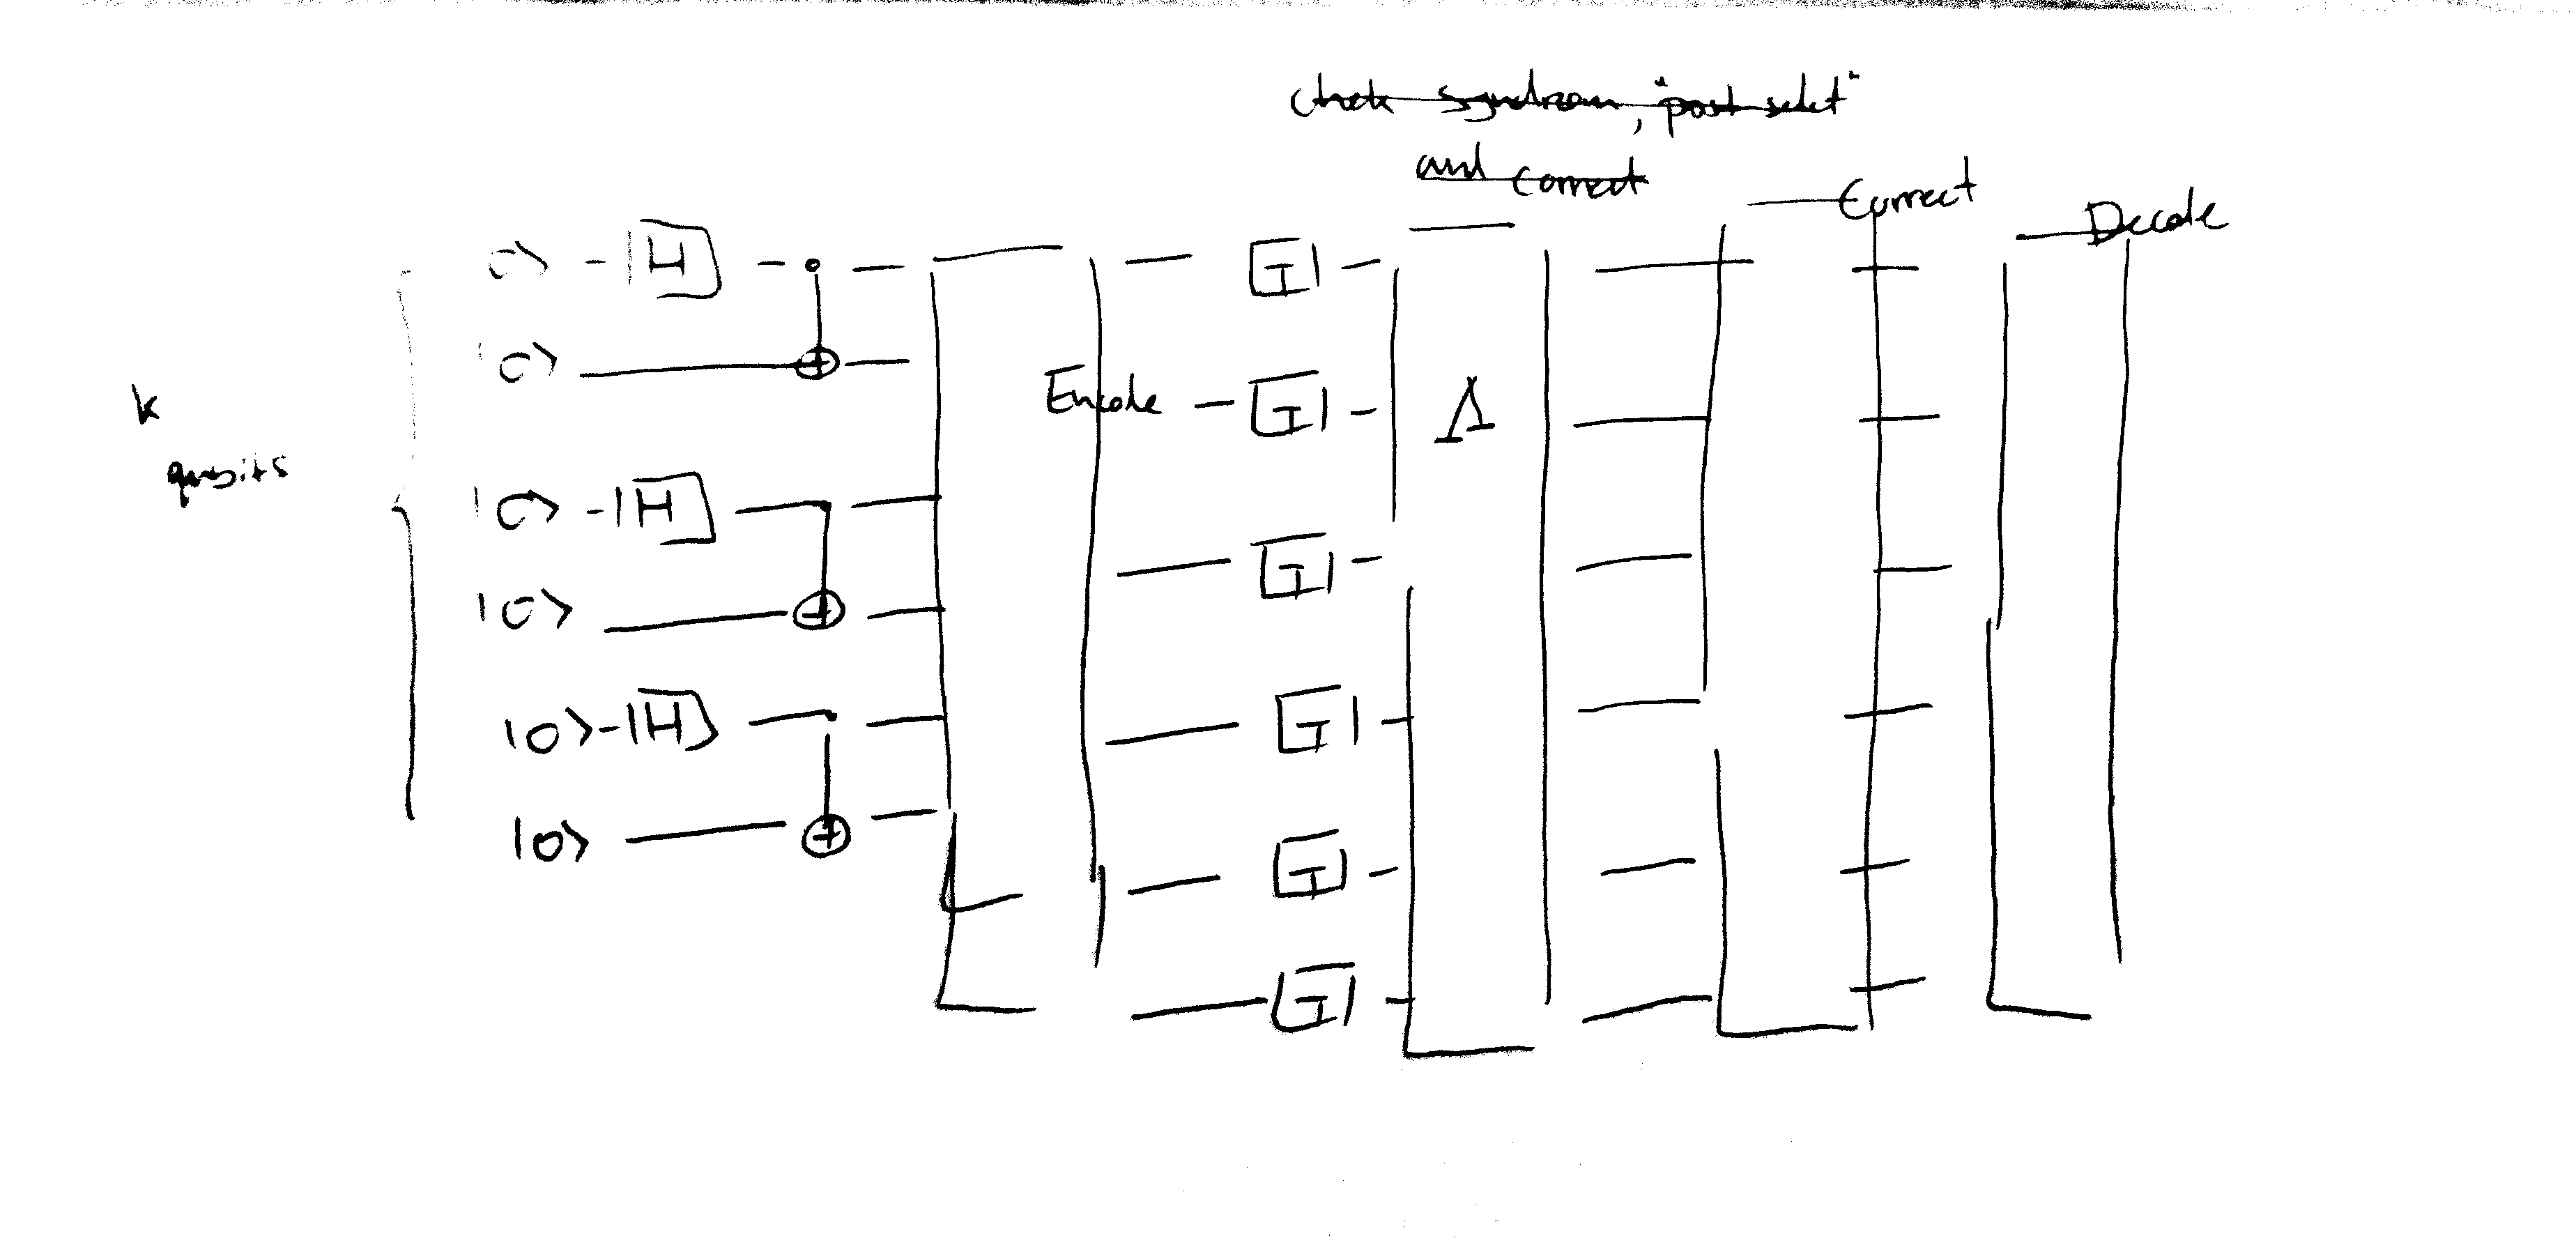
\includegraphics{distil.jpg-out.png}
}
  \caption{Quantum Circuit for distillation.}
  \label{fig:circuit}
\end{figure}

\begin{claim}
  \label{claim:phase}
  The gate $\ket{f} \mapsto \exp \Big(  -  i\pi \sum_{g,h \in G/a} X_{g}X_{h}|g\cdot h|  \Big) \ket{f} $ is in the Clifford.  
\end{claim}
\begin{proof}
Just decode $f$ and apply \textbf{CZ} between any pair of qubits corresponding to the generators $g,h$ such that $g \cap h = 1$. Then encode the state again. Observes that \textbf{CZ} is a Clifford gate, and by the fact that the code is a CSS code then the decoder and the encoder are both in the Clifford.
\end{proof}
Let's denote the circuit defined in \Cref{claim:phase} by $\Lambda$. So we have that:  
\begin{equation*}
  \begin{split}
    \Lambda^{\dagger}\exp \Big( i\pi/4 \sum_{g} X_{g}|g|  & -  i\pi \sum_{g,h \in G/a} X_{g}X_{h}|g\cdot h|  \Big) \ket{f} \\
= & \exp \Big( i\pi/4 \sum_{g} X_{g}|g|  \Big) \ket{f} 
  \end{split}
\end{equation*}

Maybe what do we need is to arrange in some way $|g|+|g^{\prime}| = 4k+1$ and $\braket{g,f}= \braket{g^{\prime},f^{\prime}}$


\begin{claim}
  For any $m$ codewords $x_{1}..x_{m}$ there is a set of coordinates $I$ and $|I| < \alpha n$. Such that:  
  \begin{equation*}
    \begin{split}
      \sum_{j \in [n]/I }x_{a}^{j}x_{b}^{j} = 0
    \end{split}
  \end{equation*}
  For any pair $x_{a},x_{b}$. 
\end{claim}

\begin{claim}
  For any $m$ codewords $x_{1}..x_{m}$ there is a set of coordinates $I$ and $|I| < \alpha n$. Such that:  
  \begin{equation*}
    \begin{split}
      \sum_{a,b,j \in [n]/I }x_{a}^{j}x_{b}^{j} = 4k
    \end{split}
  \end{equation*}
  For any pair $x_{a},x_{b}$. 
\end{claim}

\begin{claim}
  \label{claim:oneg}
  Let $C$ be a code at rate $\rho(C) > 7/8 $ has at least one codeword $x \in C$ , such that $|x| =_{8} 1 $.
\end{claim}

\begin{definition}
  We will say that a code $C$ is $(l,m)$-genorthogonal if there exists a generator set $G$ for $C$ such that for any $I \subset G$ such that $1 < |I| < l$ we have that:
  \begin{equation*}
    \begin{split}
      \sum_{i \in [n]}\prod_{g_{j}\in I \subset G}g_{j}^{i} =_{m} 0 
    \end{split}
  \end{equation*}
\end{definition}

\begin{claim}  
  If there exists a single $(l,m)$-genorthogonal code for a finite length $\Delta$, then there is a family of $(l,m)$-genorthogonal good codes. Moreover, if there exists a generator in $C_0$ of weight $|\cdot|_m = 1$, then there exists a family that also has at least one generator of weight $|\cdot|_m = 1$.
\end{claim}
\begin{proof}
  Denote by $C_{0} = \Delta[1,\rho_{0}, \delta_{0}]$ an $(l,m)$-genorthogonal code and observes that for any $C = [n,\rho n, \delta n]$ the tensor code $C_{0}\otimes C = [\Delta n, \rho_{0} \rho \Delta n, \delta_{0} \delta \Delta n]$ is also $(l,m)$-genorthogonal code. 

  For the seconed part of the claim, Choose $C$ to be a good code with rate $> \left(2^{m}-1\right)/2^{m}$ by \Cref{claim:oneg} there is at least on codeword $c$ in $C$ such that $|c| =_{m} 1$.

  So pick the base for $C_{0}\otimes C$ such the first generator is $g_{0} \otimes c$ where $g_{0}$ denote a generator of $C_{0}$ satisfies $|g_{0}| =_{m} 1$. 
    Then $|g_{0} \otimes c | = |g_{0}| \cdot |c| =_{m} 1$.  
\end{proof}

\begin{claim}
  Let $C$ be a $\rho$-rate, $(11,8)$-genorthogonal code such the generators set contains generator $c$ at weight $|c|_{8}=1$. Then there is a generators set $G^{\prime}$ for $C$ such that $C$ is $(2,8)$-genorthogonal in respeect to $G^{\prime}$ and there are at least $\rho/8$ generators $g \in G$ at weight $|g| =_{8} 1$.
\end{claim}
\begin{proof}
  If $C$ has more than $\rho/8 \cdot n$ generators at weight $| \cdot | =_{8} 1$ then we done. Otherwise by pigeonhole principle we have a $i$ such that more than $\rho/8$ portion of the generators are at weight $ |\cdot| =_{8} i$. Denote them by $g_{1},g_{2},g_{3}..g_{m}$. On the otherhand by \Cref{claim:oneg} there is in $C$ at least one codewored $c$ such that $|c| =_{8} 1$. Define the set $g_{1}^{^\prime},g_{2}^{\prime}..g_{m}^{\prime}$ as   
  \begin{equation*}
    \begin{split}
      g^{\prime}_{t} & = c + \sum_{j=t}^{t+10}g_{j} \\
      & \Rightarrow |g^{\prime}_{t+1}| = |c| + \sum_{t}{ |g_{j}| } + \sum_{|I|<10}\left|\prod_{g \in I\cup \{c\} } \alpha_{\star} g \right| \\
      & =_{8} c + 8\cdot i =_{8} c =_{8} 1  
    \end{split}
  \end{equation*} 
  On the otherhand: 
  \begin{equation*}
    \begin{split}
      g_{t}
    \end{split}
  \end{equation*}<++>
\end{proof}

\begin{claim}
  There exists, a good LDPC code (classic) $C$ such that $C^{\perp}$ is also a good code and a generator set $G$:  
  \begin{enumerate}
    \item For any pair $x \neq y \in G \rightarrow x\cdot y = 0$
    \item For any triple $x\neq y,z \in G \rightarrow \sum_{i}x_{i}y_{i}z_{i} = 0$
    \item  There exists $\rho^{\prime} > 0$ such that one can choose a generator set $G$ satisfying that at least $\rho^{\prime}$ portion of its generators $g$ have weight $|g| = 8k + 1$.
  \end{enumerate}
\end{claim}


\begin{claim} 
Let $C_0$ be a Triorthogonal code of constant length $\Delta$. Let $C_1 = [n, \rho n, \delta n]$ be a good LDPC code with rate $>7/8$ such that $C^{\perp}$ is also a good code. Denote by $C$ the hyperproduct code obtained by multiplying the tensor code defined by them. Namely:
  \begin{equation*}
    \begin{split}
      C = \left( C_{1} \otimes C_{0} \right) \times_{H} \left( C_{1} \otimes C_{0} \right)
    \end{split}
  \end{equation*} 
Then there is an efficient circuit for $2\Delta n \rightarrow (\rho_{0}\rho/8) \Delta n$ magic states distillation with asymptotic overhead approaching $1$ 
\end{claim}


\end{document}







